% Options for packages loaded elsewhere
\PassOptionsToPackage{unicode}{hyperref}
\PassOptionsToPackage{hyphens}{url}
\PassOptionsToPackage{dvipsnames,svgnames,x11names}{xcolor}
%
\documentclass[
  10pt,
]{article}
\usepackage{amsmath,amssymb}
\usepackage{iftex}
\ifPDFTeX
  \usepackage[T1]{fontenc}
  \usepackage[utf8]{inputenc}
  \usepackage{textcomp} % provide euro and other symbols
\else % if luatex or xetex
  \usepackage{unicode-math} % this also loads fontspec
  \defaultfontfeatures{Scale=MatchLowercase}
  \defaultfontfeatures[\rmfamily]{Ligatures=TeX,Scale=1}
\fi
\usepackage{lmodern}
\ifPDFTeX\else
  % xetex/luatex font selection
\fi
% Use upquote if available, for straight quotes in verbatim environments
\IfFileExists{upquote.sty}{\usepackage{upquote}}{}
\IfFileExists{microtype.sty}{% use microtype if available
  \usepackage[]{microtype}
  \UseMicrotypeSet[protrusion]{basicmath} % disable protrusion for tt fonts
}{}
\makeatletter
\@ifundefined{KOMAClassName}{% if non-KOMA class
  \IfFileExists{parskip.sty}{%
    \usepackage{parskip}
  }{% else
    \setlength{\parindent}{0pt}
    \setlength{\parskip}{6pt plus 2pt minus 1pt}}
}{% if KOMA class
  \KOMAoptions{parskip=half}}
\makeatother
\usepackage{xcolor}
\usepackage[margin=22mm]{geometry}
\usepackage{longtable,booktabs,array}
\usepackage{calc} % for calculating minipage widths
% Correct order of tables after \paragraph or \subparagraph
\usepackage{etoolbox}
\makeatletter
\patchcmd\longtable{\par}{\if@noskipsec\mbox{}\fi\par}{}{}
\makeatother
% Allow footnotes in longtable head/foot
\IfFileExists{footnotehyper.sty}{\usepackage{footnotehyper}}{\usepackage{footnote}}
\makesavenoteenv{longtable}
\usepackage{graphicx}
\makeatletter
\def\maxwidth{\ifdim\Gin@nat@width>\linewidth\linewidth\else\Gin@nat@width\fi}
\def\maxheight{\ifdim\Gin@nat@height>\textheight\textheight\else\Gin@nat@height\fi}
\makeatother
% Scale images if necessary, so that they will not overflow the page
% margins by default, and it is still possible to overwrite the defaults
% using explicit options in \includegraphics[width, height, ...]{}
\setkeys{Gin}{width=\maxwidth,height=\maxheight,keepaspectratio}
% Set default figure placement to htbp
\makeatletter
\def\fps@figure{htbp}
\makeatother
\setlength{\emergencystretch}{3em} % prevent overfull lines
\providecommand{\tightlist}{%
  \setlength{\itemsep}{0pt}\setlength{\parskip}{0pt}}
\setcounter{secnumdepth}{-\maxdimen} % remove section numbering
% definitions for citeproc citations
\NewDocumentCommand\citeproctext{}{}
\NewDocumentCommand\citeproc{mm}{%
  \begingroup\def\citeproctext{#2}\cite{#1}\endgroup}
\makeatletter
 % allow citations to break across lines
 \let\@cite@ofmt\@firstofone
 % avoid brackets around text for \cite:
 \def\@biblabel#1{}
 \def\@cite#1#2{{#1\if@tempswa , #2\fi}}
\makeatother
\newlength{\cslhangindent}
\setlength{\cslhangindent}{1.5em}
\newlength{\csllabelwidth}
\setlength{\csllabelwidth}{3em}
\newenvironment{CSLReferences}[2] % #1 hanging-indent, #2 entry-spacing
 {\begin{list}{}{%
  \setlength{\itemindent}{0pt}
  \setlength{\leftmargin}{0pt}
  \setlength{\parsep}{0pt}
  % turn on hanging indent if param 1 is 1
  \ifodd #1
   \setlength{\leftmargin}{\cslhangindent}
   \setlength{\itemindent}{-1\cslhangindent}
  \fi
  % set entry spacing
  \setlength{\itemsep}{#2\baselineskip}}}
 {\end{list}}
\usepackage{calc}
\newcommand{\CSLBlock}[1]{\hfill\break\parbox[t]{\linewidth}{\strut\ignorespaces#1\strut}}
\newcommand{\CSLLeftMargin}[1]{\parbox[t]{\csllabelwidth}{\strut#1\strut}}
\newcommand{\CSLRightInline}[1]{\parbox[t]{\linewidth - \csllabelwidth}{\strut#1\strut}}
\newcommand{\CSLIndent}[1]{\hspace{\cslhangindent}#1}
\ifLuaTeX
\usepackage[bidi=basic]{babel}
\else
\usepackage[bidi=default]{babel}
\fi
\babelprovide[main,import]{english}
% get rid of language-specific shorthands (see #6817):
\let\LanguageShortHands\languageshorthands
\def\languageshorthands#1{}
% Keep long identifiers and wide descriptive tables legible in the draft.
\emergencystretch=3em
\setlength{\tabcolsep}{3pt}
\usepackage{etoolbox}
\BeforeBeginEnvironment{longtable}{\begingroup\footnotesize}
\AfterEndEnvironment{longtable}{\endgroup}
\usepackage{float}
\floatplacement{figure}{H}
% Unicode minus in readable Markdown tables/contrasts; isolated from the old paper.
\DeclareUnicodeCharacter{2212}{\ensuremath{-}}
\usepackage{needspace}
\ifLuaTeX
  \usepackage{selnolig}  % disable illegal ligatures
\fi
\usepackage{bookmark}
\IfFileExists{xurl.sty}{\usepackage{xurl}}{} % add URL line breaks if available
\urlstyle{same}
\hypersetup{
  pdftitle={Payload-Aware Open-Set Interference Recognition for GEO Bent-Pipe Transponders},
  pdfauthor={Working manuscript --- authors and affiliations to be confirmed},
  pdflang={en},
  colorlinks=true,
  linkcolor={Maroon},
  filecolor={Maroon},
  citecolor={Blue},
  urlcolor={Blue},
  pdfcreator={LaTeX via pandoc}}

\title{Payload-Aware Open-Set Interference Recognition for GEO Bent-Pipe
Transponders}
\author{Working manuscript --- authors and affiliations to be confirmed}
\date{27 October 2026}

\begin{document}
\maketitle
\begin{abstract}
Ground monitoring of a transparent geostationary satellite observes
interference after propagation coupling, transponder filtering,
nonlinear amplification and receiver imperfections. Consequently,
waveform labels need not correspond to uniquely identifiable spectral
causes. We formulate a controlled, payload-aware open-set recognition
study that distinguishes three sources of monitoring information:
dual-polarization observations, an observation-derived cancellation
residual, and operator carrier-plan masks. A reference-model simulator
produces paired multicarrier scenes with eight known classes, three
near-family unknowns, an equivalence-limited noise family and a benign
carrier-identification control. Independent scenario roles separate
weight fitting, checkpoint selection, rejection calibration and
evaluation. Three canonical views and a separately matched plan-mask
comparison define a required fifteen-fit campaign. Unknown-positive
rankings are distinguished from known-only calibrated operating points;
uncertainty resamples whole scenario groups while retaining the trained
models and thresholds. Existing simulated visibility and cancellation
diagnostics motivate the experiment but do not establish recognition
superiority. Production-scale recognition measurements are NOT RUN, the
primary scorer is not yet researcher-designated, and prior exposure of a
small part of the preserved test population is disclosed. This draft
supplies the complete physical and statistical methods, auditable
existing evidence, and publication-ready result specifications without
presenting unexecuted comparisons as findings.
\end{abstract}

\textbf{Manuscript status.} This is the original GEO-focused
experimental manuscript, separate from the repository's
measured-GNSS/comparative-methods paper and its independent literature
review. The physical and statistical methods below are implemented or
explicitly identified as specifications. The required production-scale
recognition campaign and separately authorized final evaluation are
\textbf{NOT RUN}. Comparisons are exploratory under the accepted
statistical design: the word \emph{hypothesis} identifies a scientific
question, not a completed confirmatory superiority test. Evidence
identifiers E01--E18 resolve in \texttt{geo\_b2\_evidence.md}; its
companion JSON binds the inspected source files and reused figures by
SHA-256. This manuscript baseline is main
\texttt{6e9ff7f1c29a33e813015753cc311080da2a77ff}. No protected
observation was opened to write this draft.

\section{1. Introduction}\label{introduction}

Ground-based interference monitoring of a geostationary (GEO) bent-pipe
link is an inverse problem with an important observation boundary. An
interfering uplink can traverse the wanted satellite's input
multiplexer, amplifier and output multiplexer, whereas an interfering
signal added on the downlink can bypass that payload. Their received
spectra may nevertheless resemble one another. Transparent-channel
reference models make the ordering of these operations explicit; they do
not, by themselves, provide a unique inverse mapping from a power
spectrum to an interference source (ETSI 2014, 2021). The present study
therefore treats source recognition as a conditional statistical task
under stated observation assumptions, rather than as identification of
an orbital origin from a spectral image. {[}E01, E02{]}

Existing satellite monitoring research includes weak-interference
detection after signal cancellation, prediction of normal received
spectra, and learning from real satellite captures combined with
terrestrial interferers (Politis et al. 2017; Pellaco, Singh, and Jaldén
2019; Henarejos, Vázquez, and Pérez-Neira 2019). Thus neither applying
machine learning to satellite interference nor subtracting an estimated
desired signal is a new contribution here. The question is more
specific: which monitoring information supports recognition when weak
external signals, polarization leakage and nonlinear payload effects
coexist, and when some evaluation families were absent from classifier
training?

Operator knowledge creates a useful but easily confounded distinction
between measurements and context. Two calibrated polarization monitors
provide two spectral observations. A carrier plan states where
transmissions are expected, and, under the present receiver assumption,
their symbol rates, pulse-shaping parameters and modulation descriptors.
A cancellation residual is a derived feature computed from complex
co-polarized monitor samples and that plan. These are different
information resources. Simply comparing a model with all three resources
against a spectrum-only model would not isolate why performance changed.
Moreover, a label such as \emph{unauthorized} is defined relative to the
declared plan; a measured benefit of plan access on such labels is
partly a benefit of supplying the context used to define the task.
{[}E01--E04, E09{]}

We address three separate questions. \textbf{H1} asks whether the
canonical dual-polarization monitoring configuration improves on the
canonical co-polarization configuration. It adds the cross-polarized
spectrum \textbf{and its plan mask}, so its interpretation is
conditional on plan availability. \textbf{H2} asks whether the
co-plan-derived residual adds useful representation beyond both observed
spectra and masks. It is not a plan-independent cancellation experiment.
\textbf{H3} asks whether plan masks help when the remaining
preprocessing and training choices are matched. Its primary comparison
holds a plan-free reference and learning objective fixed and changes
only the mask channels, subject to a small input-stem parameter
difference. {[}E09{]}

Open-set recognition adds a second boundary. A classifier may be correct
among the eight trained classes yet confidently assign a nearby
untrained waveform to one of them. Conversely, a high unknown score need
not mean harmful interference: a legitimate carrier-identification
overlay is a separate benign control. Known-interference detection,
known-class recognition and unknown rejection must therefore be
evaluated with different positive classes and denominators. Open-set and
out-of-distribution methods motivate this distinction, but cannot
establish the physical meaning of a rejected RF observation (Scheirer et
al. 2013; Bendale and Boult 2016; Hendrycks and Gimpel 2017). {[}E05,
E08{]}

The bounded methodological contribution is an auditable experiment
connecting a reference-model dual-polarization payload, receiver-derived
features, near-family unknowns and information-matched comparisons. It
consists of a versioned scene model; separation of observable inputs
from simulator truth; an explicit fifteen-fit minimum design; and a
calibration and paired-analysis protocol that preserves ambiguity and
adverse outcomes. It is not a claim of first use, a new general-purpose
open-set algorithm, a measured satellite benchmark, or demonstrated
deployment performance. Existing physical diagnostics motivate the
comparisons; the article's recognition Results and outcome-dependent
Discussion remain incomplete until the declared experiments are
executed. {[}E01--E10, E16{]}

\section{2. Related Work}\label{related-work}

\subsection{2.1. Satellite interference observations and
cancellation}\label{satellite-interference-observations-and-cancellation}

Signal cancellation predates this work as a way to reveal interference
hidden beneath a wanted satellite signal (Politis et al. 2017). We use
that prior work to motivate residual-based observation, not to claim
replication of its receiver or operating point. Our monitor is on the
ground after the modeled payload and downlink, and its decision-directed
receiver is deliberately limited. Payload distortion and imperfect
reconstruction can remain in the residual alongside an interferer. A
reduction in wanted-signal power is therefore neither proof that the
interferer was preserved nor proof of better classification. The
residual must be evaluated through the explicit H2 comparison and its
physical controls. {[}E03, E11{]}

Henarejos and colleagues study learning with actual Ku-band satellite
captures and digitally combined terrestrial signals (Henarejos, Vázquez,
and Pérez-Neira 2019). Pellaco and colleagues investigate spectrum
prediction and deviation detection with received satellite spectra
(Pellaco, Singh, and Jaldén 2019). These studies prevent an overly broad
claim that previous satellite learning uses only simulation. They also
illustrate why the injection point matters: digitally combining received
signals is not the same experiment as propagating an uplink interferer
through the wanted nonlinear transponder. We distinguish those
observation domains without inferring that one domain universally yields
harder or easier recognition. {[}E02, E18{]}

On-board CNN interference detection and NGSO-to-GSO detection provide
further satellite-specific comparisons of representation and learning
methods (Daoud et al. 2023; Saifaldawla et al. 2024). Their published
task definitions and associated source descriptions do not establish a
common eight-known-class, dual-polarization, ground-monitor open-set
benchmark with the present carrier-plan assumptions. Consequently, their
performance numbers are not imported into our tables. A method-level
numerical comparison would require compatible observations, labels,
splits and lawful data access; no such new comparison is claimed here.
{[}E18{]}

\subsection{2.2. Payload models and observation
fidelity}\label{payload-models-and-observation-fidelity}

ETSI's DVB-S2 reference channel describes the transparent
IMUX--amplifier--OMUX structure, while the implementation guidelines
provide reference filter data (ETSI 2014, 2021). We use the repository's
derived filter responses and digitized nonlinear TWTA curves as
traceable reference models. Saleh's classical nonlinear amplifier model
is an available analytical alternative, not the default payload
substituted into the headline experiment (Saleh 1981). Reference-curve
agreement is a consistency target; it is not validation against a newly
measured satellite.

The physical coupling model preserves coherent complex mixing between
polarization feeds before and after two separate nonlinear paths. Its
unitary Jones approximation and effective-linewidth phase-noise model
are stated assumptions, rather than full antenna, propagation or
oscillator characterizations. Independent instrument calibration
corrects the modeled monitor response while retaining propagation
leakage. This distinction is necessary to avoid a calibration procedure
that inadvertently removes the impairment used to define a class.
{[}E02{]}

\subsection{2.3. Open-set learning and RF
interpretation}\label{open-set-learning-and-rf-interpretation}

Open-set recognition formalizes the need to reject inputs outside the
trained class set (Scheirer et al. 2013). OpenMax is an established deep
open-set approach (Bendale and Boult 2016); it is related work, not an
implemented baseline in this campaign. Maximum softmax probability is a
simple confidence baseline (Hendrycks and Gimpel 2017), energy scores
provide a logit-based alternative (Liu et al. 2020), and
class-conditional feature distances motivate Mahalanobis scoring (Lee et
al. 2018). These scores are compared as fixed post-hoc constructions. We
do not reproduce Lee and colleagues' complete
multi-layer/input-preprocessing detector, nor train the energy model
with auxiliary outliers. {[}E07, E08{]}

Residual learning motivates the compact convolutional backbone (He et
al. 2016), and center loss motivates training a class-structured
embedding (Wen et al. 2016). Our architecture is a small task-specific
residual network, not an ImageNet ResNet replica. Our center term uses a
batch mean of summed squared distances and optimizes centers with AdamW;
its scaling and update rule differ from the original center-loss
algorithm. Neither the backbone nor this adapted loss is presented as a
novel learning algorithm. The research contribution depends on the
physical experiment and fair information contrasts, whose outcomes are
still pending. {[}E07, E09{]}

Rejection also requires disciplined interpretation. The present
calibrated threshold is an empirical known-validation quantile, not a
distribution-free guarantee or a conformal predictor. An unknown-family
ranking is not a calibrated operating point, and a simulator root-cause
label is not proof that the cause is identifiable from the available
observation. These distinctions guide the metrics, controls and
limitations below. {[}E01, E08, E10{]}

\section{3. GEO Bent-Pipe Physical System
Model}\label{geo-bent-pipe-physical-system-model}

\subsection{3.1. Paired multicarrier scenes and transparent
payload}\label{paired-multicarrier-scenes-and-transparent-payload}

Let the two nominal uplink feeds be indexed by \(p\in\{c,x\}\). Their
complex signals are

\[x_p(t)=\sum_{m\in\mathcal P_p}a_{pm}s_{pm}(t)e^{j2\pi f_{pm}t},\]

where \(\mathcal P_p\) is the declared operator plan and each \(s_{pm}\)
is a pulse-shaped modulated carrier. QPSK, 8PSK, 16APSK and 32APSK are
supported within the repository waveform conventions. This
representation does not implement complete DVB-S2 framing, coding, pilot
tracking or a standards-compliant modem. The scene generator binds
plans, carrier streams, noise streams, link settings, oscillator
realizations and missing-carrier state to one scenario group. Class
variants share these quantities and alter the registered event. Any
infeasible common carrier placement is handled by a bounded, recorded
redraw; unexpected simulator errors propagate rather than silently
removing difficult scenes. {[}E01--E03{]}

Writing \(\mathbf x=[x_c,x_x]^T\), a compact expression for the
simulated observation is

\[\begin{aligned}
\mathbf v(t)&=\mathbf J_d\,\mathbf F\!\left[e^{j\phi_s(t)}\mathbf J_u\big(\mathbf x(t)+\mathbf i_u(t)+\mathbf n_u(t)\big)\right]+\mathbf i_d(t),\\
\mathbf z(t)&=\widehat{\mathbf H}^{-1}\!\left[\mathbf H e^{j\phi_r(t)}\mathbf v(t)+\mathbf n_r(t)\right].
\end{aligned}\]

The operator \(\mathbf F\) applies an IMUX, fixed-gain nonlinear
amplifier and OMUX separately to each feed. \(\mathbf J_u\) and
\(\mathbf J_d\) describe physical uplink and downlink coupling;
\(\mathbf H\) is the instrument response and \(\widehat{\mathbf H}\) its
independently estimated calibration. This equation is a block-order
description, not a claim that nonlinear multicarrier propagation reduces
to a linear matrix channel. The same symbol \(\mathbf n_r\) includes the
receiver/downlink thermal-noise convention used by the implementation.
Its per-feed reference is the pre-downlink-mixing OMUX output, and
inverse instrument correction transforms that noise as well as the
wanted signal. {[}E02{]}

The default filters and TWTA are derived reference responses (ETSI 2014,
2021). Input back-off is referenced to the configured saturation
convention, not inferred by the classifier. Fixed gain is retained when
a planned carrier is absent: active power falls and realized back-off
changes. Renormalizing the surviving carriers would remove a physical
consequence of the missing-carrier event and would define a different
experiment. Overdrive acts on the co-feed payload drive; an uplink
interferer enters before coupling and payload processing, whereas the
registered downlink ASI event is added after physical downlink mixing
and bypasses the wanted payload. {[}E01, E02, E05{]}

\subsection{3.2. Polarization, phase noise and instrument
calibration}\label{polarization-phase-noise-and-instrument-calibration}

The symmetric coupling matrix is

\[\mathbf J=\begin{bmatrix}c&e^{j\psi}s\\-e^{-j\psi}s&c\end{bmatrix},\qquad c^2+s^2=1,\quad c^2/s^2=10^{\mathrm{XPD}/10}.\]

This unitary approximation conserves total instantaneous power under
ideal basis mixing. XPD describes isolated-source co/cross
discrimination; the aggregate ratio of two simultaneously loaded
monitored feeds is not an XPD estimate. Uplink and downlink mixing
generally do not commute with the nonlinear feed-wise payload. Nominal
uplink/downlink XPDs of 30/35 dB, instrument XPD of 25 dB and the 10 dB
uplink fault are declared model settings. They are not sampled
measurements of a particular satellite fleet or a measured distribution
of polarization faults. {[}E02{]}

Two independent Wiener phase processes represent a common satellite
oscillator and a common receiver oscillator, each shared across both
polarizations. For effective linewidth \(\beta\),

\[\operatorname{Var}[\phi(t+\Delta t)-\phi(t)]=2\pi\beta\Delta t.\]

The registered linewidths are 100 and 50 Hz. Gap increments connect the
sparsely retained snapshots without simulating every skipped high-rate
sample. This effective Lorentzian description is not a measured
single-sideband phase-noise mask and does not represent rain
depolarization, arbitrary frequency-dependent antenna leakage or all
receiver synchronization impairments. Static calibration is not
oscillator phase tracking. {[}E02{]}

Independent full-rank complex pilots fit
\(\mathbf Y=\mathbf H\mathbf X\) by least squares, with rank and
conditioning checks before inversion. The baseline uses 64 pilot samples
with synthetic complex-noise standard deviation 0.001. Instrument gains
and phases are specified in the configuration; only their estimate is
used for correction, not the true response matrix. Physical propagation
coupling remains in the calibrated scene. These are simulated
calibration measurements, not evidence that a real dual-polarization
ground station has been calibrated. {[}E02{]}

\textbf{Table 1. Frozen baseline settings. Values are simulation choices
unless expressly identified as a reference-model structure.}

\begin{longtable}[]{@{}
  >{\raggedright\arraybackslash}p{(\columnwidth - 4\tabcolsep) * \real{0.3333}}
  >{\raggedright\arraybackslash}p{(\columnwidth - 4\tabcolsep) * \real{0.3333}}
  >{\raggedright\arraybackslash}p{(\columnwidth - 4\tabcolsep) * \real{0.3333}}@{}}
\toprule\noalign{}
\begin{minipage}[b]{\linewidth}\raggedright
Quantity
\end{minipage} & \begin{minipage}[b]{\linewidth}\raggedright
Baseline / range
\end{minipage} & \begin{minipage}[b]{\linewidth}\raggedright
Interpretation
\end{minipage} \\
\midrule\noalign{}
\endhead
\bottomrule\noalign{}
\endlastfoot
Channel / simulation / monitor bandwidth-rate & 36 MHz / 288 MS/s / 96
MS/s & Finite sampled reference channel \\
Snapshots / spacing / retained IQ & 128 / 10 ms / 4096 samples per
snapshot & Sparse schedule, not contiguous 1.28 s IQ \\
PSD bins / bin spacing & 512 / 187.5 kHz & Monitor grid spans 96 MHz \\
Nominal IBO / overdrive IBO & 9--13 dB / 1--4 dB & Fixed-gain payload
convention \\
Uplink and downlink C/N & 15--30 dB per path & Declared noise-reference
conventions \\
Uplink / downlink / instrument XPD & 30 / 35 / 25 dB & Nominal settings,
not measured distributions \\
Cross-polarization fault & Uplink XPD 10 dB & Controlled impairment \\
Satellite / receiver linewidth & 100 / 50 Hz & Effective Wiener model \\
Planned-carrier omission & Probability 0.15 per group & One carrier
across the two feeds; recorded conditioning \\
\end{longtable}

Settings and references: E01--E03. The temporal span describes when
short windows are observed; interpreting it as a continuous long record
would overstate the available information.

\subsection{3.3. Registered interference
taxonomy}\label{registered-interference-taxonomy}

The eight known labels are simulator root causes, with at most one
primary event per variant. The independent auxiliary target concerns
carrier absence, not an additional primary interference label. Table 2
records which physical intervention defines each known class. This
distinction prevents interpreting labels as universal spectral
categories. {[}E01, E03{]}

\textbf{Table 2. Known classes and primary interventions. C/I
denominators must be retained.}

\begin{longtable}[]{@{}
  >{\raggedright\arraybackslash}p{(\columnwidth - 4\tabcolsep) * \real{0.3333}}
  >{\raggedright\arraybackslash}p{(\columnwidth - 4\tabcolsep) * \real{0.3333}}
  >{\raggedright\arraybackslash}p{(\columnwidth - 4\tabcolsep) * \real{0.3333}}@{}}
\toprule\noalign{}
\begin{minipage}[b]{\linewidth}\raggedright
Class
\end{minipage} & \begin{minipage}[b]{\linewidth}\raggedright
Intervention
\end{minipage} & \begin{minipage}[b]{\linewidth}\raggedright
Registered level or distinction
\end{minipage} \\
\midrule\noalign{}
\endhead
\bottomrule\noalign{}
\endlastfoot
Clean & Nominal loaded link & May still have the independent
missing-carrier state \\
CW & Co-feed uplink tone & Total-plan C/I 5--35 dB \\
Swept CW & Co-feed swept tone & C/I 5--35 dB; sweep span 1 MHz--0.9
channel bandwidth \\
Unauthorized & Modulated carrier in a plan gap & PSD relative to plan
mean: −10 to +3 dB \\
Overdrive & Co-feed payload drive & IBO 1--4 dB \\
Cross-pol & Increased uplink coupling & Uplink XPD changed to 10 dB \\
Uplink ASI & Carrier traversing wanted payload & Geometry-derived PSD
C/I; 20--80\% plan overlap \\
Carrier-under-carrier & Carrier inside an active victim band &
Total-plan C/I 5--30 dB \\
\end{longtable}

The ASI construction uses a simplified single-interferer,
common-coverage uplink budget,
\(C/I_{\rm PSD}=G_{\max}-G(\varphi)-\Delta\mathrm{EIRP}_{\rm density}\),
with documented reference antenna-pattern branches and explicitly
assumed diameter, pointing and EIRP distributions. Its natural level
distribution differs from that of the gap carrier. Consequently, high
natural-distribution classification accuracy for the ASI/unauthorized
pair could reflect level rather than the overlap cue. The dedicated
level-matched set is necessary to examine that shortcut; natural and
matched results answer different questions. {[}E01, E06, E12{]}

The three near-family unknowns are pulsed CW, intermittent CW bursts and
downlink ASI. They share mechanisms with trained classes and are
deliberately not portrayed as distant arbitrary anomalies. Wideband
noise is reported separately because it can be observationally
equivalent to an elevated uplink noise floor. The benign
\texttt{cid\_overlay} places carrier-identification signals under
transmitted co-feed carriers and has expected decision \emph{clean}; it
is excluded from unknown-positive pooling. No test-only family or its
outcomes is used as a surrogate unknown for fitting or threshold choice.
{[}E05{]}

\section{4. Payload-Aware Recognition
Methodology}\label{payload-aware-recognition-methodology}

\subsection{4.1. Spectral inputs and information
access}\label{spectral-inputs-and-information-access}

The canonical stored observation contains calibrated spectra
\(S_c,S_x\in\mathbb R^{128\times512}\), plan masks
\(M_c,M_x\in\mathbb R^{512}\) and a co-feed residual spectrum
\(R_c\in\mathbb R^{128\times512}\). Spectra, masks and residuals are
stored as float16 and converted to float32 model inputs during
preprocessing. Spectral values are dB of simulated power density, not
calibrated field dBm. Masks are broadcast along time and retain their
separate relative-level meaning. Time pooling averages linear powers
before converting to dB. The frozen pooling factor two yields 64 time
positions; spectra are clipped to {[}−60, 20{]} dB relative to their
reference and scaled by 20. These fixed conventions are not selected
from test performance. {[}E03, E07{]}

The canonical reference is each scene's observed co-feed mean linear PSD
over the co-plan core, defined by mask values above −3 dB, converted to
dB. Both polarizations and the residual use this \textbf{same}
reference. Independent normalization of the feeds would change the
relative-level cue H1 examines. This per-scene carrier reference itself
uses the plan, so removing only mask input channels would leave a
plan-information path in an alleged plan-independent control. {[}E07,
E09{]}

The canonical views are \(X_{\rm co}=[S_c,M_c]\),
\(X_{\rm dual}=[S_c,S_x,M_c,M_x]\) and
\(X_{\rm residual}=[S_c,S_x,M_c,M_x,R_c]\), after their declared
preprocessing. Simulator truth such as realized IBO, XPD, C/I, source
identity, active-carrier masks and event parameters remains metadata for
auditing or registered stratification. It is never a learned input.
Conditioning plots on such metadata does not turn it into an
operationally available detector feature. {[}E01, E03, E07{]}

\subsection{4.2. Observation-derived carrier
cancellation}\label{observation-derived-carrier-cancellation}

The frozen receiver is P20 \texttt{obs-cancel/1}. It consumes calibrated
co-feed IQ and declared carrier descriptors: center frequency, symbol
rate, roll-off, modulation and the APSK code-rate/ring-ratio identifier.
Availability and accuracy of those descriptors are monitoring
assumptions. The receiver does not receive transmitted symbols, true
activity, event labels or payload settings. It processes every planned
carrier, including a carrier that is physically absent. {[}E03{]}

For each short monitor block, the receiver resamples to the simulation
rate, mixes each planned carrier to baseband and applies a unit-energy
SRRC matched filter spanning ten symbols. Oerder--Meyr timing estimation
is quantized to the high-rate grid. A 16-point coarse phase search over
the modulation symmetry sector initializes hard decisions, followed by
three decision-directed complex least-squares gain iterations. The
reconstructed carriers are remodulated, summed, decimated and subtracted
from the observed co-feed signal:

\[r_c[n]=z_c[n]-\sum_{m\in\mathcal P_c}\widehat z_{cm}[n].\]

The learned fifth channel is the residual PSD, not the reconstructed
symbols or receiver diagnostics. No nonlinear inverse of the TWTA is
assumed. {[}E03{]}

An edge guard removes 512 monitor samples at each end. The residual
therefore uses 3072 samples and eleven Welch segments, versus fifteen
segments from 4096 samples for the original spectrum. Identical density
scaling and frequency bins do not imply identical estimator variance.
Decision errors, filter-induced ISI, cross-polarization leakage, finite
boundaries and phase walk remain in the residual. A block-constant
complex gain cannot track the frozen phase process within the block; the
later theoretical analysis gives phase-noise-only limits around
21.7/22.8 dB for full/guarded windows, not imposed clipping values or
measured universal ceilings. {[}E03, E04{]}

The separate P21b \texttt{B2-features/1} receiver includes fractional
timing and a short received-domain FIR and uses a different center-loss
convention. It is not silently substituted for P20 and is not a
single-variable H2 comparator. Likewise, an oracle event-free twin used
in a diagnostic is not part of the operational cancellation input. H2
tests a receiver-derived representation from observed complex IQ and the
plan; it does not assert that a deterministic transformation creates
information beyond its original IQ inputs. {[}E03, E04, E11{]}

\subsection{4.3. Classifier, objective and fixed training
recipe}\label{classifier-objective-and-fixed-training-recipe}

A full-resolution \(5\times5\) stem feeds four residual stages. Global
mean and maximum pooling are concatenated into a \(D=16w\) embedding,
followed by an eight-class linear head and, for canonical models, an
independent binary auxiliary head. At width \(w=16\), \(D=256\). At
width 16, canonical co/dual/residual model parameter counts are
310,505/311,305/311,705, excluding separately learned class centers. H1
and H2 therefore change input-stem capacity as well as the available
representation. Retaining the initial frequency grid lets a narrow
spectral line reach a nonlinearity before downsampling; maximum pooling
complements the global mean. This is an architectural rationale rather
than an observed improvement over another backbone. {[}E07{]}

For a training batch of size \(B\), with embedding \(f_i\), class center
\(c_{y_i}\) and physical missing-carrier indicator \(a_i\), the
canonical objective is

\[\mathcal L=\mathcal L_{\rm CE}+0.005\,\frac1B\sum_i\|f_i-c_{y_i}\|_2^2+1.0\,\mathcal L_{\rm BCE}(\widehat a_i,a_i).\]

The center sum is not divided by embedding dimension and has no
additional one-half factor. Centers share the network's AdamW parameter
group and weight decay. This is an explicitly frozen adaptation of
center-loss learning (Wen et al. 2016). The auxiliary positive class is
a physically absent planned carrier, \(a=1\); it is not general
operator-plan/spectrum agreement. Classifier selection uses only primary
known-class validation macro-F1, not auxiliary performance. {[}E07,
E10{]}

The approved recipe uses exactly 30 epochs, batch 32, width 16, time
pooling two, peak learning rate \(10^{-3}\), weight decay \(10^{-4}\),
and the existing cosine OneCycle schedule with cycled momentum. There is
no early stopping, clipping, autocast or automatic batch reduction. Both
matmul and cuDNN TF32 are explicitly off for FP32 training; this does
not promise bit-exact GPU determinism. Train groups alone provide 12,000
known observations and 11,250 optimizer steps per fit. Four-group shards
and four-shard blocked-shuffle windows bound memory, with batch
remainders carried across windows. Blocked shuffling is not global
sample shuffling. {[}E07, E10{]}

Canonical training retains shared-channel mirror/time-roll augmentation
and K17b plan-mask shift: each training sample is selected with
probability 0.15 and shifted continuously within ±0.5 MHz. Both masks
move together and normalization is recomputed from the shifted plan,
while the stored spectrum and cancellation residual remain unchanged.
Validation, calibration and final-test masks are unshifted in the main
experiment. This augmentation addresses one belief error; it is not
equivalent to recomputing cancellation with a wrong receiver descriptor.
{[}E05, E07, E10{]}

\section{5. Open-Set Detection and
Calibration}\label{open-set-detection-and-calibration}

\subsection{5.1. Scores and training-only fitted
state}\label{scores-and-training-only-fitted-state}

The known prediction is \(\widehat y=\arg\max_k z_k\) for eight logits
\(z_k\). Three unknown scores are reported, always with larger values
meaning more unknown-like:

\[s_{\rm MSP}=1-\max_k\operatorname{softmax}(\mathbf z)_k,\qquad s_E=-\log\sum_k e^{z_k},\]

\[s_M=\min_k(f-\mu_k)^T\widetilde\Sigma^{-1}(f-\mu_k).\]

MSP and energy follow established confidence constructions (Hendrycks
and Gimpel 2017; Liu et al. 2020). Temperature is fixed at one, without
unknown-informed temperature tuning. Energy is sensitive to a common
logit offset, unlike MSP, so native score magnitudes are not compared
across unrelated models. For Mahalanobis scoring, each \(\mu_k\) and the
pooled within-class covariance are fitted from training embeddings only;
no validation or unknown embedding enters their estimation. {[}E08{]}

Specifically, \(\Sigma\) uses class-centered residuals and denominator
\(\max(N-K,1)\), and

\[\widetilde\Sigma=0.9\Sigma+0.1\frac{\operatorname{tr}\Sigma}{D}I+\delta I,\qquad \delta=\max\!\left(10^{-6}\frac{\operatorname{tr}\Sigma}{D},10^{-8}\right).\]

Distances use a Cholesky solve. This single-embedding,
shrinkage-regularized score is related to feature-distance detection
(Lee et al. 2018), not an exact reproduction of its complete procedure.
A positive diagonal floor ensures numerical invertibility even when
within-class variability is poorly estimated; it does not establish that
a tiny training pilot supplies reliable covariance statistics. {[}E08{]}

Mahalanobis is the current \textbf{recommendation}, motivated by the
center-structured embedding, but is \textbf{NOT DESIGNATED} as primary
by the researcher. All three scores remain reported regardless of the
eventual pre-test designation. Neither favorable pilot ranks nor final
held-out outcomes may be used to select the headline scorer
retrospectively. {[}E09, E10{]}

\subsection{5.2. Independent rejection and clean-alarm
calibration}\label{independent-rejection-and-clean-alarm-calibration}

Each scorer has its own threshold from the known-only \texttt{val-calib}
role. For ordered calibration scores \(u_{(0)}\le\cdots\le u_{(n-1)}\),
the empirical \texttt{higher} 0.95 quantile is

\[\tau=u_{(\lceil0.95(n-1)\rceil)}.\]

A sample is accepted as known when \(s\le\tau\) and rejected when
\(s>\tau\). Equality is accepted; ties and finite calibration
populations affect realized acceptance. The target 0.95 known acceptance
is not a population guarantee, and pooled calibration does not impose
95\% acceptance within every known class. Thresholds are specific to the
fitted model, score and calibration artifact, and cannot be transported
across views merely because their target is identical. {[}E08, E10{]}

A separate clean-versus-event alarm uses
\(s_A=\sum_{k\ne\mathrm{clean}}p_k\), mathematically
\(1-p_{\mathrm{clean}}\) but evaluated without subtractive saturation.
Its threshold uses \textbf{clean} \texttt{val-calib} observations only,
the same \texttt{higher} rule at 0.95, and a strict greater-than alarm.
This targets clean false-alarm probability 0.05 and differs from
rejection of an untrained family. In particular, known interference is
positive for event detection but negative for an unknown-positive ROC
calculation. {[}E08, E10{]}

\subsection{5.3. Ranking, operating points and
uncertainty}\label{ranking-operating-points-and-uncertainty}

The primary endpoint is near-family pooled unknown-positive FPR@95TPR
for the canonical residual view. It is the fraction of known test
observations at or above the first grouped-score threshold attaining at
least 95\% detection of the pooled near-family unknowns. Equal-score
observations enter the ranking curve together; this ranking convention
differs from strict greater-than rejection at a calibrated operating
point. Known negatives include all eight classes, including known
interference. This is an evaluation ranking summary whose threshold is
determined by the ranked test scores; it is \textbf{not} the
known-validation calibrated threshold or an operational threshold
selected for deployment. Lower FPR@95TPR is better. AUROC, average
precision, OSCR and fixed-threshold rejection/acceptance complete the
picture. {[}E05, E08--E10{]}

For OSCR, the known correct-classification rate counts observations that
are both accepted and correctly classified, divided by \textbf{all}
known test observations. The paired horizontal quantity is the fraction
of all unknown test observations accepted as known. Merely accepting a
known sample is not correct recognition. AP depends on the pooled
prevalence: the complete near-family population has 1,500 unknown
observations against 4,000 known observations, whereas a single-family
row has 500 unknowns against the same 4,000 knowns. The wideband-noise
and benign-CID controls are separate populations. Closed-set macro-F1,
per-class recall and confusion are computed without pretending that a
binary event detector predicts eight classes. {[}E05, E08{]}

Intervals resample whole scenario groups, preserving their paired class
variants and unknown families. The same bootstrap resample is shared
across compared arms and seeds. These percentile intervals condition on
the frozen weights, feature statistics and thresholds; they do not
include training, calibration, simulator or field-distribution
uncertainty. Seeds 0, 1 and 2 are reported separately with a descriptive
mean and spread, not a three-seed confidence claim. The accepted design
does not support a confirmatory superiority claim or unadjusted
multiplicity inference from many class/bin/scorer comparisons. Empty or
undefined metrics remain unavailable with counts and reasons; they are
never encoded as zero success. {[}E09, E10{]}

\section{6. Experimental Design and
Ablations}\label{experimental-design-and-ablations}

\subsection{6.1. Scenario roles, pairing and
exposure}\label{scenario-roles-pairing-and-exposure}

\textbf{Table 3. Full intended populations. Counts describe the frozen
generator, not completed production.}

\begin{longtable}[]{@{}
  >{\raggedright\arraybackslash}p{(\columnwidth - 6\tabcolsep) * \real{0.2143}}
  >{\raggedleft\arraybackslash}p{(\columnwidth - 6\tabcolsep) * \real{0.2857}}
  >{\raggedleft\arraybackslash}p{(\columnwidth - 6\tabcolsep) * \real{0.2857}}
  >{\raggedright\arraybackslash}p{(\columnwidth - 6\tabcolsep) * \real{0.2143}}@{}}
\toprule\noalign{}
\begin{minipage}[b]{\linewidth}\raggedright
Role
\end{minipage} & \begin{minipage}[b]{\linewidth}\raggedleft
Groups
\end{minipage} & \begin{minipage}[b]{\linewidth}\raggedleft
First group ID
\end{minipage} & \begin{minipage}[b]{\linewidth}\raggedright
Observations / use
\end{minipage} \\
\midrule\noalign{}
\endhead
\bottomrule\noalign{}
\endlastfoot
Train & 1500 & 3000000 & 12,000 known; weights and feature statistics \\
Validation-selection & 150 & 3100000 & 1,200 known; checkpoint selection
only \\
Validation-calibration & 150 & 3150000 & 1,200 known; rejection and
clean alarm \\
Natural test & 500 & 3200000 & 4,000 known + 2,500 test-only/control
variants \\
Level-matched test & 150 & 3300000 & 450 clean/ASI/unauthorized
variants \\
\end{longtable}

The total is 21,350 observations: 18,400 known variants across the four
known roles, 2,500 test-only/control variants and 450 matched variants.
Registration here means versioned repository commitments and dated
researcher decisions, not registration in an independent external
registry. Every group remains in one role. Sharing carrier/noise and
event-control realizations across a group's variants is deliberate
pairing, not independent replication. The group, rather than each of its
eight images, is the resampling unit. Unknown families are excluded from
training, checkpoint selection, feature-statistic fitting and
calibration. {[}E01, E03, E05, E06, E10{]}

The preserved test population is \textbf{not pristine}. Groups
3200000/3200001 and matched groups 3300000/3300001 were exposed in
earlier pilots; group 3200000 also has a committed observation-derived
display. Every final report must therefore retain the 500/150-group
headline and show 498/148-group sensitivity rows excluding those IDs,
without choosing exclusions by outcomes. This disclosure cannot prove
that earlier exposure had no influence on design decisions. It instead
makes that limitation auditable and prevents a false claim that
freeze-before-read erases historical access. This manuscript reads only
already committed summaries and figures. {[}E10{]}

\subsection{6.2. H1, H2 and H3 as distinct
estimands}\label{h1-h2-and-h3-as-distinct-estimands}

\textbf{Table 4. Registered contrasts. The sign is richer minus
comparator; negative FPR@95TPR differences favor the richer arm.}

\begin{longtable}[]{@{}
  >{\raggedright\arraybackslash}p{(\columnwidth - 6\tabcolsep) * \real{0.2500}}
  >{\raggedright\arraybackslash}p{(\columnwidth - 6\tabcolsep) * \real{0.2500}}
  >{\raggedright\arraybackslash}p{(\columnwidth - 6\tabcolsep) * \real{0.2500}}
  >{\raggedright\arraybackslash}p{(\columnwidth - 6\tabcolsep) * \real{0.2500}}@{}}
\toprule\noalign{}
\begin{minipage}[b]{\linewidth}\raggedright
Question
\end{minipage} & \begin{minipage}[b]{\linewidth}\raggedright
Required contrast
\end{minipage} & \begin{minipage}[b]{\linewidth}\raggedright
Held fixed / changed
\end{minipage} & \begin{minipage}[b]{\linewidth}\raggedright
Interpretation limit
\end{minipage} \\
\midrule\noalign{}
\endhead
\bottomrule\noalign{}
\endlastfoot
H1 & Dual − co & Same canonical recipe; adds cross PSD and cross mask &
Dual monitoring with plans, not isolated spectrum-only information \\
H2 & Dual-residual − dual & Same canonical recipe; adds co-plan-derived
residual & Plan-conditional receiver representation \\
H3 & Dual-planmask − dual-noplan & Same plan-free reference/objective;
adds two masks & Mask-access benefit, with a small stem-capacity
difference \\
\end{longtable}

For H3, both arms use one fixed reference: the training mean of the
per-observation 90th frequency percentile of time-averaged co-feed PSD
\textbf{in dB}. They share that plan-independent scalar at validation
and test time. Neither arm uses the auxiliary plan-consistency objective
or plan-shift augmentation, and neither uses a residual. The no-plan
path drops mask/residual arrays before preprocessing and rejects
plan-derived settings. This closes information paths that would remain
if one merely hid the mask channels of a canonically normalized model.
The control is global-reference plan-independent, not a stronger
per-scene plan-free normalization variant that was never added to the
required roster. {[}E07, E09{]}

The two matched arms share seeds, data order, augmentation streams,
optimizer/schedule, center-loss convention and all non-stem tensor
initialization. The different input dimensionality necessarily changes
the first convolution; at width 16 the dual mask arm has 800 additional
stem parameters. Equal nominal width is therefore not exact parameter
equality. The initialization procedure re-seeds non-stem modules
independently of stem shape, preventing an avoidable RNG-order confound.
Relative to the canonical recipe, both matched arms change exactly three
declared settings: fixed plan-free rather than per-scene carrier
reference, no auxiliary plan head, and no plan shift. Consequently,
canonical dual minus dual-planmask is only a descriptive decomposition,
and canonical dual minus dual-noplan does not isolate mask value.
{[}E09{]}

For a metric \(m\), the paired seed-specific effect is
\(\Delta_{h,s}=m(\text{richer}_{h,s})-m(\text{comparator}_{h,s})\). Both
point estimates and bootstrap differences use aligned populations and
the frozen scorer designation. Selection of a favorable seed, scorer,
subgroup or optional arm after viewing protected results is excluded. A5
plan corruption tests sensitivity of an already trained plan-using
system; it does not replace H3's learned, matched plan-access
comparison. Likewise, H1 without plans would require the optional
co-noplan fits, which are not part of the fifteen-fit minimum. {[}E09,
E10{]}

\subsection{6.3. Near-family and level-matched
controls}\label{near-family-and-level-matched-controls}

Downlink ASI reuses the known uplink ASI group's event draw so that
geometry, modulation, rate, roll-off, placement and requested PSD C/I
are paired. Injection before versus after the wanted payload is the
intended distinction. However, the downlink event is scaled by realized
wanted-feed power while uplink interference uses nominal unit loading. A
missing co-feed carrier therefore creates a registered level drift; this
is not an ideal all-conditions level-matched causal intervention. The
accepted generator-derived metadata identify 35 co-feed missing groups
and their 465-group complement; 43 cross-feed drops make 78 drops in
total. The 500/35/465 report is distinct from the 500/498 exposure
sensitivity. The later production metadata comparison is mandatory and
\textbf{NOT RUN}. {[}E05, E10{]}

The separate ASI/unauthorized set uses 150 groups with shared requested
\(C/I_{\rm PSD}\sim U(4,13)\) dB, symbol rate, roll-off, modulation and
link conditions, alongside a clean twin. Its primary bin is 7--10 dB,
with 4--7 and 10--13 dB neighboring bins. Frequency placement remains
different by class definition: overlap versus free gap. Equal requested
injected power does not force equal observed PSD rise, because the clean
background and nonlinear interactions differ between the two bands.
Results must retain full pair-class denominators, including
clean/other-known predictions and rejected samples; conditioning only on
predictions of the two desired classes could conceal failure. {[}E06{]}

Joint placement feasibility also conditions the matched population: its
carrier rates are at most 6 Mbaud, whereas natural test-role ASI spans
1--28.8 Mbaud, and the matched 10--13 dB bin extends beyond the natural
unauthorized level range. An ASI variant can overlap a planned but
physically absent carrier, so its relation to actual transmitted
occupancy must be reported separately. P22's metadata-only pre-draw
found this intersection in 5 of 150 groups; that count is not a
completed production observation measurement. These limitations prevent
equating natural-versus-matched changes with a pure level intervention,
even when the two arms within a matched group share requested power.
{[}E06{]}

Additional registered interpretation controls include CuC level bins
5--15, 15--25 and 25--30 dB; noise/back-off stratification; benign CID
clean acceptance and false CuC calls; and overdrive scenes whose
out-of-plan regrowth remains below the clean-calibrated threshold. These
are mechanism-specific views of the same frozen predictions, not
opportunities to change labels after observing difficulty. Source truth
may define reporting strata but is not an extra model input.
Receiver-consistent plan-error experiments, full leave-one-known-out
sweeps, alternative cyclic features and linear-to-nonlinear transfer
remain outside the minimum campaign; none has a newly executed result
here. {[}E01, E06, E10, E14{]}

\subsection{6.4. Required fits and pre-test
freeze}\label{required-fits-and-pre-test-freeze}

The minimum roster is nine canonical fits,
\(\{\mathrm{co,dual,dual\_residual}\}\times\{0,1,2\}\), and six matched
dual fits, \(\{\mathrm{dual\_planmask,dual\_noplan}\}\times\{0,1,2\}\).
Optional matched co-planmask/co-noplan fits would add six and are
deferred. They must not be chosen after the first protected result.
Thirty epochs are run completely; the first highest primary validation
macro-F1 selects the checkpoint. An interrupted production fit is
incomplete and restarts from epoch zero in a fresh attempt rather than
splicing optimizer, scheduler or RNG state. {[}E09, E10, E16{]}

Before any separately authorized final observation read, the campaign
binds all fifteen checkpoint, scorer and calibrator identities, selected
epochs, configuration, population/role identity, source and effective
runtime, the researcher's primary-scorer designation, and the fixed
canonical-then-H3-dual evaluation sequence. The optional co controls are
recorded as deferred. A scorer designation is not itself permission to
read data. Current code provides the campaign admission/custody
interface, but the separately authorized production held-out inference
integration remains absent. The present manuscript neither implements
that reader nor opens the protected set. {[}E16{]}

\section{7. Existing Simulated Evidence and Results
Specifications}\label{existing-simulated-evidence-and-results-specifications}

\subsection{7.1. What has actually been
measured}\label{what-has-actually-been-measured}

The observations in Table 5 are already committed \textbf{simulation
diagnostics}, not new experiments and not measured satellite data. They
motivate questions about available cues without answering H1--H3. The
older single-polarization runs omit the later dual-polarization and
phase-noise blocks; P20 cancellation uses a different population. Their
numerical values are not combined into a common detector comparison.
Exact aggregate pointers and figure hashes are supplied in E11--E13.
{[}E11--E13{]}

\textbf{Table 5. Existing physical evidence, with its observation
boundary.}

\begin{longtable}[]{@{}
  >{\raggedright\arraybackslash}p{(\columnwidth - 6\tabcolsep) * \real{0.2500}}
  >{\raggedright\arraybackslash}p{(\columnwidth - 6\tabcolsep) * \real{0.2500}}
  >{\raggedright\arraybackslash}p{(\columnwidth - 6\tabcolsep) * \real{0.2500}}
  >{\raggedright\arraybackslash}p{(\columnwidth - 6\tabcolsep) * \real{0.2500}}@{}}
\toprule\noalign{}
\begin{minipage}[b]{\linewidth}\raggedright
Diagnostic
\end{minipage} & \begin{minipage}[b]{\linewidth}\raggedright
Existing population
\end{minipage} & \begin{minipage}[b]{\linewidth}\raggedright
Recorded quantity
\end{minipage} & \begin{minipage}[b]{\linewidth}\raggedright
Permitted interpretation
\end{minipage} \\
\midrule\noalign{}
\endhead
\bottomrule\noalign{}
\endlastfoot
Natural uplink ASI & 120 single-pol groups; IBO 11 dB; C/N 25 dB; no
phase noise & Median PSD C/I 20.3 dB & Result of the assumed geometry
distribution \\
CuC at total-plan C/I 20 / 30 dB & 24 paired single-pol groups at each
level; same fixed link & Median twin PSD contrast 0.373 / 0.041 dB &
Weak spectral cue under this model; no Pd estimate \\
P20 cancellation & 64 observations, 8 groups across four roles & Class
mean active-core depth 12.78--16.47 dB & Receiver behavior; not
full-band depth or recognition \\
P20 CuC twin contrast & Same 8 groups & Median 0.986 to 6.461 dB
before/after; 8/8 increase & Offline truth-selected victim-band
diagnostic \\
\end{longtable}

The event/no-event contrast is
\(10\log_{10}(\overline P_{\rm event}/\overline P_{\rm twin})\) in a
diagnostic region. The twin and truth-selected victim band are
unavailable to a live monitor. The ASI PSD C/I and CuC total-plan C/I
denominators are different and must not share an unlabeled horizontal
axis. At high C/I, a small twin contrast motivates testing alternative
representations, but does not prove an information-theoretic
impossibility or a neural detection probability. {[}E11, E12{]}

\begin{figure}
\centering
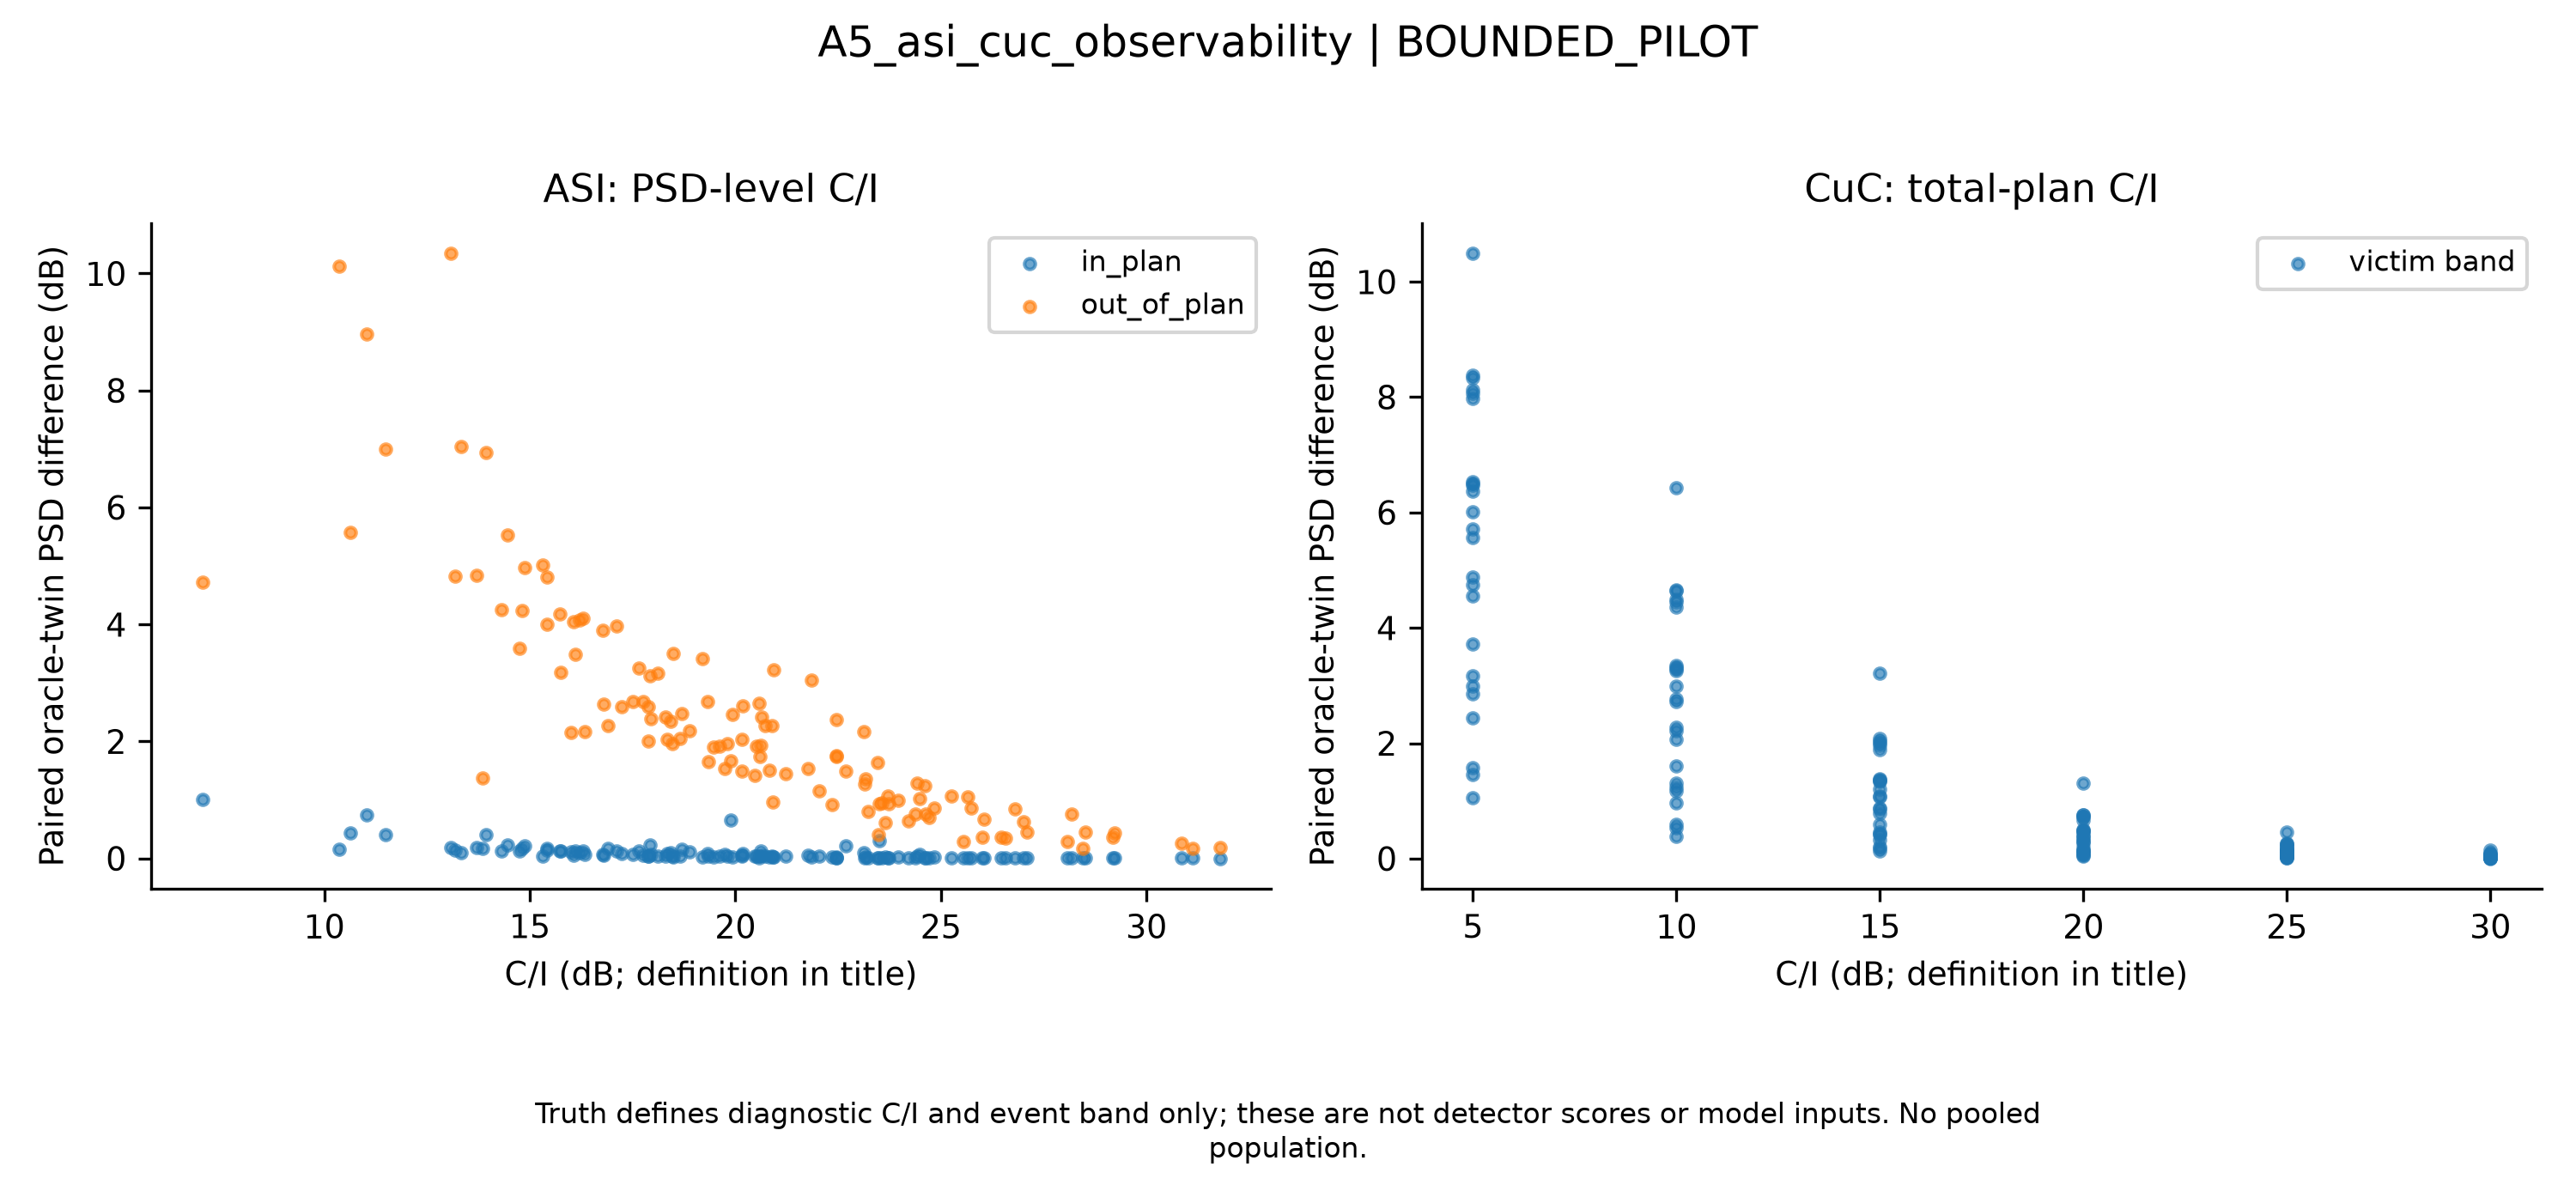
\includegraphics[width=0.95\textwidth,height=\textheight]{figures/asi_cuc_observability.png}
\caption{Reused physical visibility diagnostics, not recognition
results. ASI uses 120 single-polarization groups and PSD-referenced C/I;
CuC uses 24 groups at each level and total-plan C/I. Both use the older
fixed IBO 11 dB, uplink/downlink C/N 25 dB configuration without phase
noise. Contrasts use paired event-free twins and diagnostic bands that
are not operational model inputs. The panels have different interference
references and are not a common detector-performance curve. Reused
byte-for-byte from the validated figure package; E12--E13.}
\end{figure}

\begin{figure}
\centering
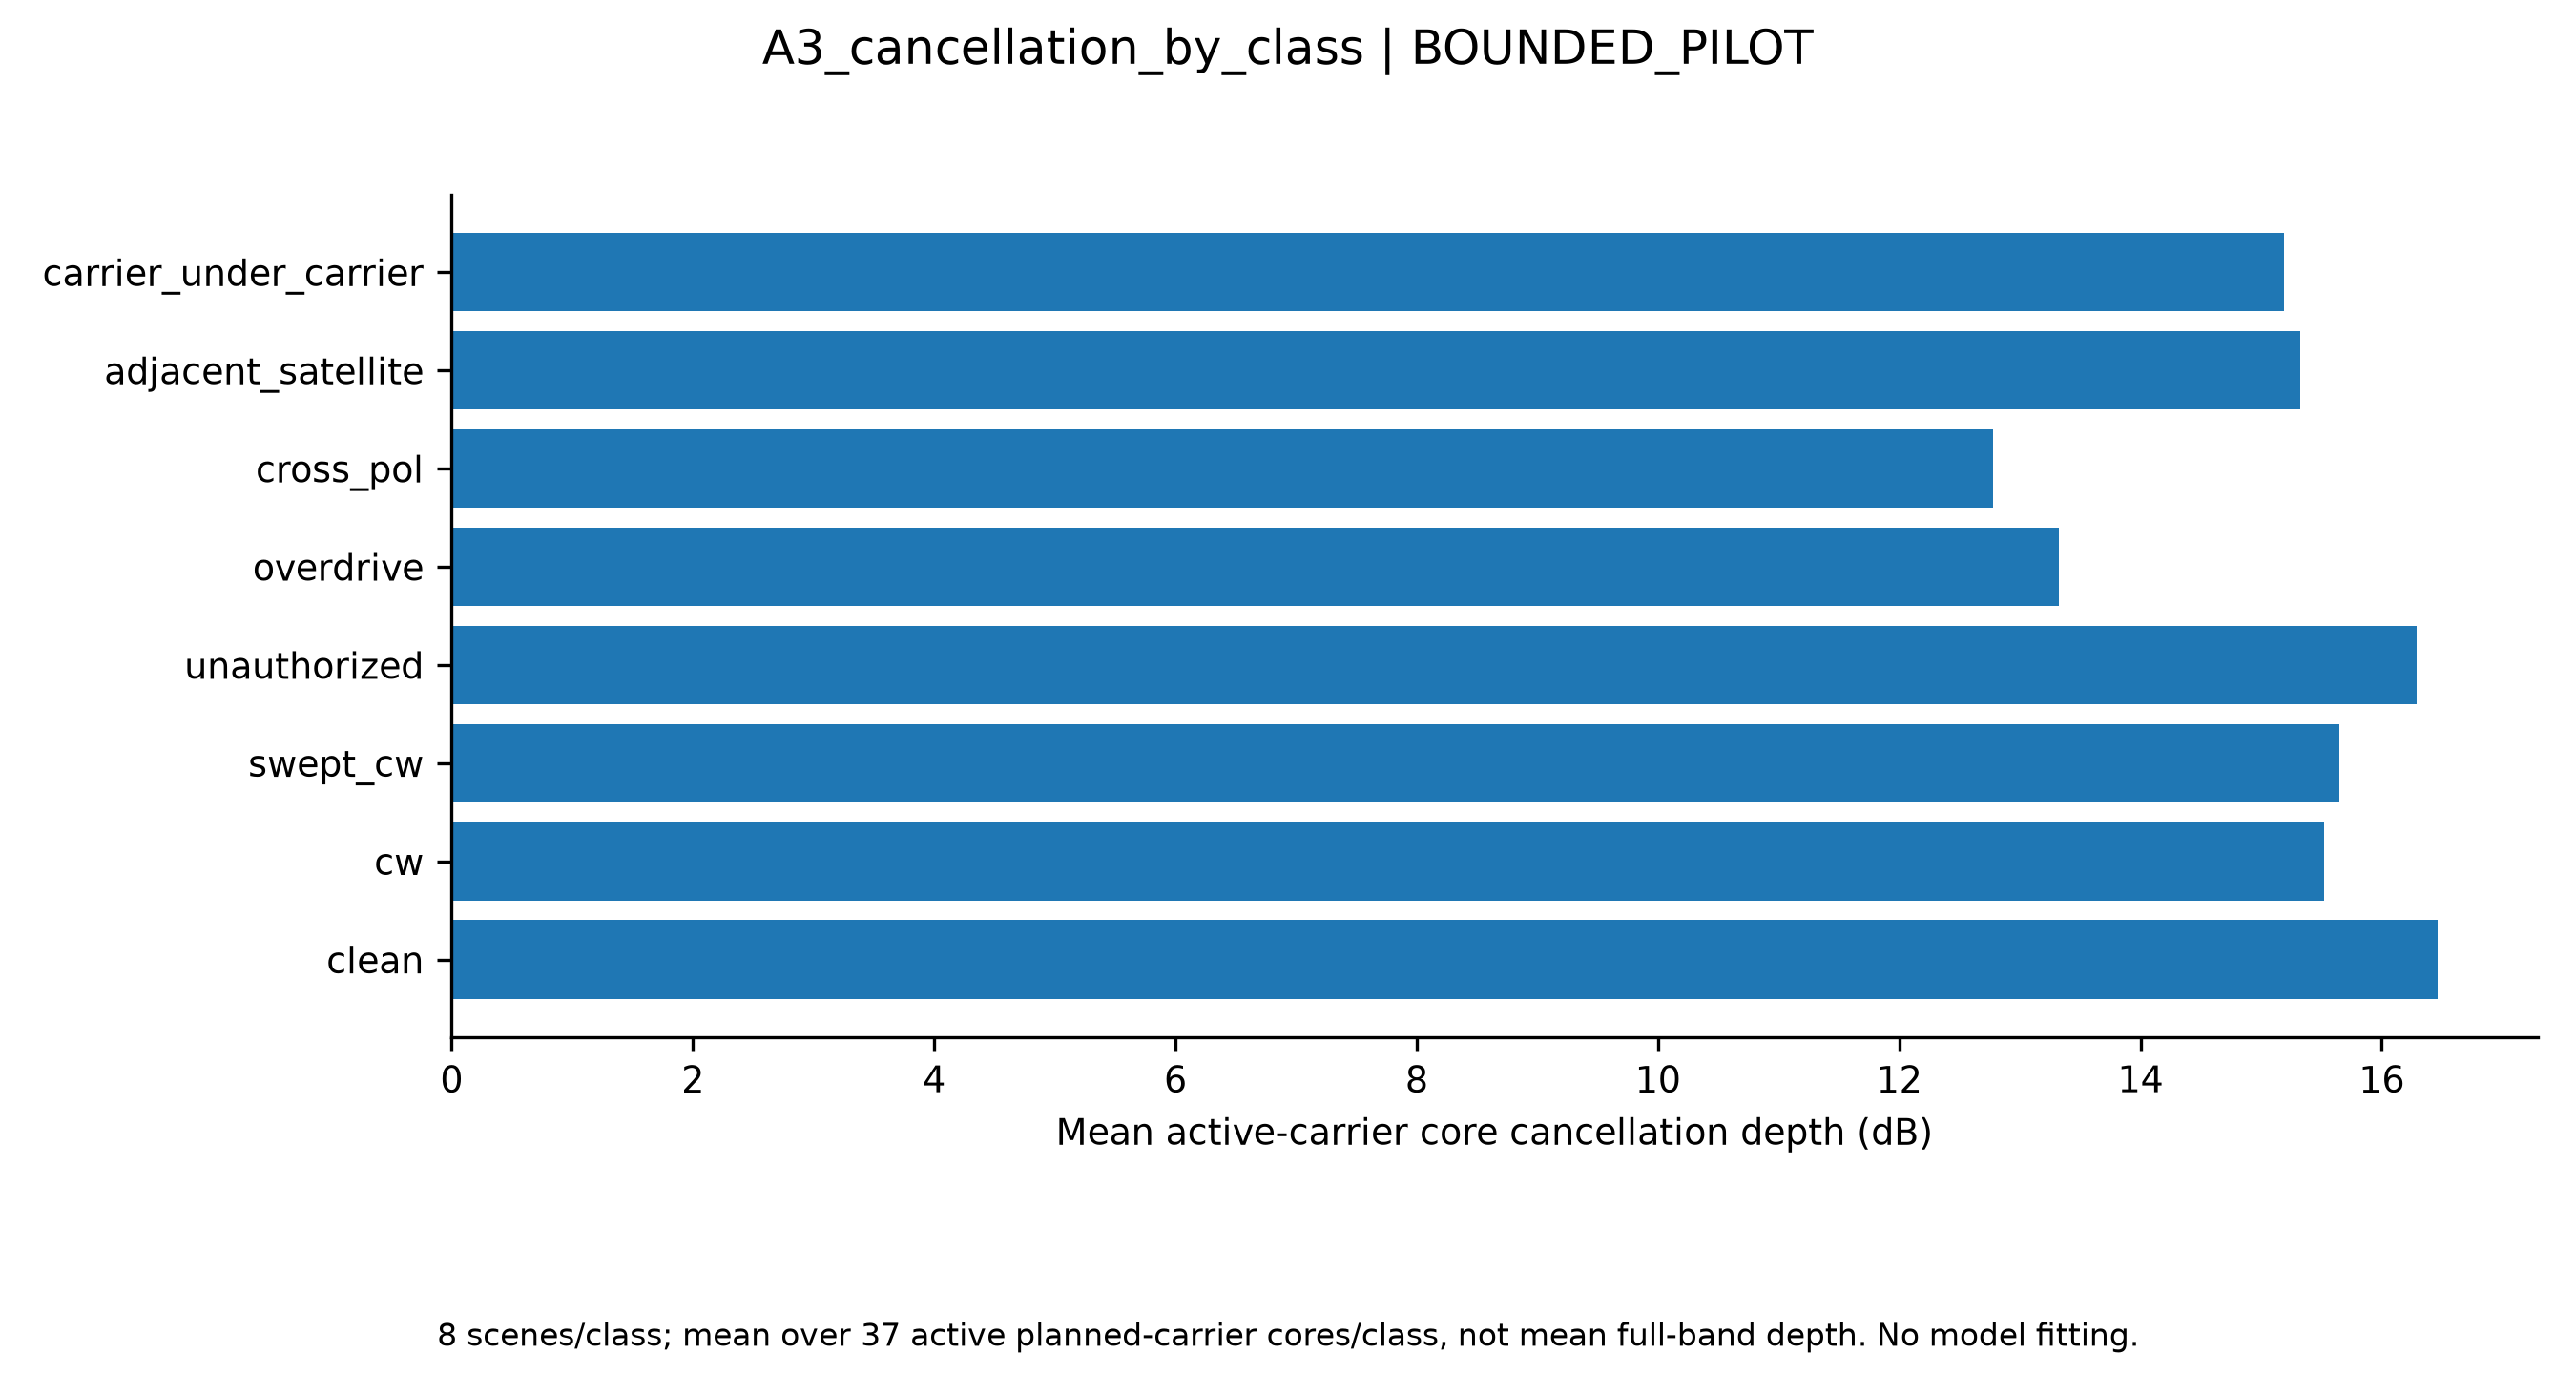
\includegraphics[width=0.95\textwidth,height=\textheight]{../docs/figures/b2/A3_cancellation_by_class.png}
\caption{Existing P20 class-wise cancellation diagnostic: 64
observations in eight paired groups across four roles, eight
observations per class and 37 active planned-carrier cores per class.
Mean occupied-core PSD reduction is not full-band cancellation depth, Pd
or recognition improvement. The historical diagnostic included test-role
pilot groups; that exposure is disclosed, and this draft reuses only the
committed aggregate figure. The bars are class means; no confidence
interval is displayed. Reused byte-for-byte; E11, E13.}
\end{figure}

Historical small neural pilots include chance-level/degenerate
predictions and uninformative auxiliary accuracy where no positive
missing-carrier cases occurred. Bounded train/calibrate/freeze and C2
invariance exercises verify data flow and control isolation, not
relative recognition quality. They are not substituted for any entry in
the following production tables. In particular, neither a favorable
physical residual contrast nor a successful checkpoint reload supplies
an observed H2 effect. {[}E09, E11, E15{]}

\subsection{7.2. Production recognition results --- NOT
RUN}\label{production-recognition-results-not-run}

\textbf{Table 6. Required fit inventory and publication table skeleton.
Every measurement cell is explicitly NOT RUN. All three scorers must be
retained; ``primary'' remains NOT DESIGNATED.}

\begin{longtable}[]{@{}
  >{\raggedright\arraybackslash}p{(\columnwidth - 10\tabcolsep) * \real{0.1667}}
  >{\raggedright\arraybackslash}p{(\columnwidth - 10\tabcolsep) * \real{0.1667}}
  >{\raggedright\arraybackslash}p{(\columnwidth - 10\tabcolsep) * \real{0.1667}}
  >{\raggedright\arraybackslash}p{(\columnwidth - 10\tabcolsep) * \real{0.1667}}
  >{\raggedright\arraybackslash}p{(\columnwidth - 10\tabcolsep) * \real{0.1667}}
  >{\raggedright\arraybackslash}p{(\columnwidth - 10\tabcolsep) * \real{0.1667}}@{}}
\toprule\noalign{}
\begin{minipage}[b]{\linewidth}\raggedright
View
\end{minipage} & \begin{minipage}[b]{\linewidth}\raggedright
Seeds
\end{minipage} & \begin{minipage}[b]{\linewidth}\raggedright
Known accuracy / macro-F1
\end{minipage} & \begin{minipage}[b]{\linewidth}\raggedright
Near FPR95: MSP
\end{minipage} & \begin{minipage}[b]{\linewidth}\raggedright
Near FPR95: energy
\end{minipage} & \begin{minipage}[b]{\linewidth}\raggedright
Near FPR95: Mahalanobis
\end{minipage} \\
\midrule\noalign{}
\endhead
\bottomrule\noalign{}
\endlastfoot
Co & 0, 1, 2 separately & NOT RUN & NOT RUN & NOT RUN & NOT RUN \\
Dual & 0, 1, 2 separately & NOT RUN & NOT RUN & NOT RUN & NOT RUN \\
Dual-residual & 0, 1, 2 separately & NOT RUN & NOT RUN & NOT RUN & NOT
RUN \\
Dual-planmask & 0, 1, 2 separately & NOT RUN & NOT RUN & NOT RUN & NOT
RUN \\
Dual-noplan & 0, 1, 2 separately & NOT RUN & NOT RUN & NOT RUN & NOT
RUN \\
\end{longtable}

The final table expands every seed into its own row and adds a
separately labeled descriptive mean/spread. Companion tables must
provide AUROC/AP/OSCR, known acceptance, accepted-known accuracy,
unknown rejection and clean false alarms with numerators and
denominators. Exposure-excluded and K17d rows retain separate labels.
The linked display specification defines populations, axes and
aggregation without inventing measurements. {[}E09, E10, E17{]}

\Needspace{9\baselineskip}

\textbf{Table 7. Paired hypothesis-effect skeleton. Units are percentage
points for FPR95; intervals condition on fixed fitted state.}

\begin{longtable}[]{@{}
  >{\raggedright\arraybackslash}p{(\columnwidth - 10\tabcolsep) * \real{0.1667}}
  >{\raggedright\arraybackslash}p{(\columnwidth - 10\tabcolsep) * \real{0.1667}}
  >{\raggedright\arraybackslash}p{(\columnwidth - 10\tabcolsep) * \real{0.1667}}
  >{\raggedright\arraybackslash}p{(\columnwidth - 10\tabcolsep) * \real{0.1667}}
  >{\raggedright\arraybackslash}p{(\columnwidth - 10\tabcolsep) * \real{0.1667}}
  >{\raggedright\arraybackslash}p{(\columnwidth - 10\tabcolsep) * \real{0.1667}}@{}}
\toprule\noalign{}
\begin{minipage}[b]{\linewidth}\raggedright
Contrast
\end{minipage} & \begin{minipage}[b]{\linewidth}\raggedright
Seed 0
\end{minipage} & \begin{minipage}[b]{\linewidth}\raggedright
Seed 1
\end{minipage} & \begin{minipage}[b]{\linewidth}\raggedright
Seed 2
\end{minipage} & \begin{minipage}[b]{\linewidth}\raggedright
Descriptive seed mean
\end{minipage} & \begin{minipage}[b]{\linewidth}\raggedright
Paired group-bootstrap interval
\end{minipage} \\
\midrule\noalign{}
\endhead
\bottomrule\noalign{}
\endlastfoot
H1: dual − co & NOT RUN & NOT RUN & NOT RUN & NOT RUN & NOT RUN \\
H2: dual-residual − dual & NOT RUN & NOT RUN & NOT RUN & NOT RUN & NOT
RUN \\
H3: dual-planmask − dual-noplan & NOT RUN & NOT RUN & NOT RUN & NOT RUN
& NOT RUN \\
\end{longtable}

These are publication specifications, not empty evidence for a favorable
direction. A positive, negative, null-looking or uncertain effect must
be retained as observed. Ranking metrics and clean-calibrated operating
metrics can disagree and require separate interpretation.
Outcome-dependent Discussion is deliberately unwritten: no claim about
which information source helps is justified until Table 7 and the
corresponding operating-point/ambiguity controls are populated. {[}E09,
E17{]}

\subsection{7.3. Minimum experiments to complete Results and
Discussion}\label{minimum-experiments-to-complete-results-and-discussion}

First, after separate execution authorization under the frozen
protocols, generate and verify the known, test-only/control and
level-matched artifacts, retaining the distinct populations and
metadata-only D8 cross-check. Second, execute the fifteen declared
30-epoch fits, select on validation-selection, fit feature statistics
from train only, calibrate on known validation-calibration and freeze
every fitted object. Third, fix the primary scorer and evaluation order
before the first separately authorized protected read, then evaluate
canonical and H3-dual inventories once using the same natural and
matched populations. Fourth, compute the offline paired contrasts and
the required exposure, K17d, class/level and benign-CID reports, and
populate the defined tables/figures with counts and conditional
uncertainty. No additional fit is required for these reporting strata.
{[}E09, E10, E16, E17{]}

These are the minimum experiments for the \textbf{narrow H1--H3
manuscript}, not completion of every historical B2 extension. Full LOKO,
SCF, amplifier-transfer/C3 and receiver-level plan-error studies must
remain labeled unexecuted unless separately specified and authorized.
The optional co-only H3 controls are not silently added to the headline.
If future authors claim superiority to CFAR, EDSC or expert-feature
classifiers, those comparators must also be run on the identical frozen
production populations; bounded historical baseline figures cannot
supply that comparison. The current draft makes no such superiority
claim. {[}E01, E09, E14, E17{]}

\section{8. Threats to Validity and
Reproducibility}\label{threats-to-validity-and-reproducibility}

\subsection{8.1. Physical and construct
validity}\label{physical-and-construct-validity}

The simulator implements a controlled reference channel, not a
calibrated digital twin of a named GEO payload. Digitization and finite
FIR responses limit the filter/amplifier representation. The Jones
approximation excludes general lossy or frequency-dependent coupling;
effective Wiener linewidths are not measured oscillator spectra. Assumed
geometry, pointing and loading distributions do not establish
operational prevalence. The experiment addresses conditional behavior
within those assumptions, and field transfer requires independent
measured evidence. Results from measured GNSS or solid-state PA tasks
are not inserted as validation of this GEO recognition system. {[}E02,
E12, E18{]}

Root-cause labels can exceed what is identifiable in the selected
observable. Weak CuC, noise-floor changes and nominal-looking overdrive
are deliberate hard cases. ASI/unauthorized placement is defined
relative to a plan, while a downlink event can resemble an uplink event
despite a different causal path. Better classification under the
simulator may exploit correlates of its sampling rules. It does not
establish unique source attribution, authorization judgment without an
operator plan, or identification of an interfering satellite. The
level-matched and missing-carrier controls expose specific confounds;
they do not exhaust all possible shortcuts. {[}E01, E05, E06, E12{]}

\subsection{8.2. Receiver and information-assumption
validity}\label{receiver-and-information-assumption-validity}

Cancellation assumes accurate carrier descriptors and shares
waveform/constellation conventions with the simulator. P20 records
unresolved APSK start-angle standard verification and grid-aligned
timing conditions; self-consistency should not be presented as
independent modem validation. A stronger real receiver might track phase
and equalize better; a real monitor with stale descriptors might perform
worse. Neither direction is established here. H2 measures this
particular representation and receiver. H1 also changes plan-mask
access, and H3 retains a small stem-capacity difference and a global,
rather than per-scene, plan-free reference. These delimit the estimated
effects even if the resulting tables show a large gap. {[}E02--E04,
E09{]}

Plan-mask augmentation is especially easy to overinterpret. Its stored
residual is fixed, whereas an erroneous receiver plan can change
cancellation itself. Historical A5 diagnostics distinguish mask-only and
receiver-consistent interventions, but their tiny chance-level models do
not establish robust recognition. A plan sensitivity claim requires its
own receiver-consistent experiment and cannot be inferred from H3 or
from a no-change argmax in an execution pilot. {[}E04, E09, E14{]}

\subsection{8.3. Statistical validity and prior
exposure}\label{statistical-validity-and-prior-exposure}

Paired variants are dependent by design, calibration is finite and three
training seeds are a small sample. Group bootstrap intervals condition
on already selected/fitted objects and omit several sources of
uncertainty. Numerous scorers, families, bins and contrasts increase
interpretive flexibility. All fixed scores and adverse outcomes must be
reported; seed averages are descriptive and no post-hoc winner is
promoted. The 95\% known-acceptance target and 5\% clean-alarm target do
not guarantee test behavior, while FPR@95TPR summarizes a different
thresholding question. {[}E08--E10{]}

Historical test exposure is a material limitation, not a footnote cured
by a new artifact hash. Both complete and identity-excluded sensitivity
populations are required, and neither replaces the separately labeled
co-feed-missing analysis. A sign-consistent result across these rows
would improve interpretability but would not retroactively create an
untouched external test. Subsequent design changes motivated by final
outcomes require new, prospectively separated evidence rather than
rebranding the current test population. {[}E10{]}

\subsection{8.4. Reproducibility, artifacts and
access}\label{reproducibility-artifacts-and-access}

Generator requests bind source, configuration, role populations,
calibration and checksummed shards. Training and calibration markers
bind data, source, runtime and fitted-state identities; stale
checkpoints are rejected instead of relabeled. Effective
Torch/CUDA/cuDNN/device/driver and TF32 settings must be recorded for
production execution. An interrupted fit is incomplete, and no missing
or unavailable measurement is interpreted as zero. Such provenance makes
a result auditable; it cannot establish that the assumed physical model
is true or that a storage device survived an untested failure. {[}E03,
E07, E10, E16{]}

This manuscript package contains Markdown, bibliography, traceability
records, document-only validation/build tools and reused aggregate
figures. It requires no raw IQ, protected dataset, checkpoint, simulator
run or fitting operation to build. The existing comparative-methods
manuscript and independent literature review remain separate and
unchanged. Public primary references establish cited method identities
and bounded prior-work statements, while the source audit records
full-text versus metadata-only access. Authors, affiliations, venue
suitability and publication approval remain human decisions. No claim of
systematic literature completeness or priority is made. {[}E13, E16,
E18{]}

\section{9. Conclusion}\label{conclusion}

The scientific question is how explicitly stated observation resources
change a fixed open-set GEO recognition task, rather than whether a
single architecture can label every possible interference cause. The
proposed experiment separates dual-monitor access, a plan-conditioned
receiver residual and mask access under matched preprocessing. Its role
isolation, known-only calibration, near-family grouping and paired
analyses provide a concrete basis for answering those questions.
Existing physical diagnostics explain why the questions are nontrivial;
they do not answer them. Production-scale recognition results, the
primary-scorer designation and final protected evaluation remain
pending. The manuscript is therefore a substantive methods-and-design
draft with honest evidence boundaries, ready for completion by the
specified experiments rather than by invented performance claims.
{[}E01--E18{]}

\section{References}\label{references}

\phantomsection\label{refs}
\begin{CSLReferences}{1}{0}
\bibitem[\citeproctext]{ref-bendale2016openmax}
Bendale, Abhijit, and Terrance E. Boult. 2016. {``Towards Open Set Deep
Networks.''} In \emph{Proceedings of the IEEE Conference on Computer
Vision and Pattern Recognition}, 1563--72.
\url{https://doi.org/10.1109/CVPR.2016.173}.

\bibitem[\citeproctext]{ref-daoud2023dataset}
Daoud, Saed, Geoffrey Eappen, Flor Ortiz, Eva Lagunas, Wallace Martins,
and Symeon Chatzinotas. 2023. {``{CNN}-Based on-Board Interference
Detection in Satellite Systems: An Analysis of Dataset Impact on
Performance.''} In \emph{2023 IEEE International Conference on
Acoustics, Speech, and Signal Processing Workshops (ICASSPW)}, 1--5.
\url{https://doi.org/10.1109/ICASSPW59220.2023.10193395}.

\bibitem[\citeproctext]{ref-etsi2014dvbs2}
ETSI. 2014. {``{EN 302 307-1 V1.4.1}: Digital Video Broadcasting
({DVB}); Second Generation Framing Structure, Channel Coding and
Modulation Systems; Part 1: {DVB-S2}.''}
\url{https://www.etsi.org/deliver/etsi_en/302300_302399/30230701/01.04.01_60/en_30230701v010401p.pdf}.

\bibitem[\citeproctext]{ref-etsi2021dvbs2guide}
---------. 2021. {``{TR 102 376-2 V1.2.1}: Digital Video Broadcasting
({DVB}); Implementation Guidelines for the Second Generation System;
Part 2: {S2} Extensions ({DVB-S2X}).''}
\url{https://www.etsi.org/deliver/etsi_tr/102300_102399/10237602/01.02.01_60/tr_10237602v010201p.pdf}.

\bibitem[\citeproctext]{ref-he2016resnet}
He, Kaiming, Xiangyu Zhang, Shaoqing Ren, and Jian Sun. 2016. {``Deep
Residual Learning for Image Recognition.''} In \emph{Proceedings of the
IEEE Conference on Computer Vision and Pattern Recognition}, 770--78.
\url{https://www.cv-foundation.org/openaccess/content_cvpr_2016/html/He_Deep_Residual_Learning_CVPR_2016_paper.html}.

\bibitem[\citeproctext]{ref-henarejos2019interference}
Henarejos, Pol, Miguel Ángel Vázquez, and Ana Isabel Pérez-Neira. 2019.
{``Deep Learning for Experimental Hybrid Terrestrial and Satellite
Interference Management.''} \url{https://arxiv.org/abs/1906.03012}.

\bibitem[\citeproctext]{ref-hendrycks2017baseline}
Hendrycks, Dan, and Kevin Gimpel. 2017. {``A Baseline for Detecting
Misclassified and Out-of-Distribution Examples in Neural Networks.''} In
\emph{International Conference on Learning Representations}.
\url{https://arxiv.org/abs/1610.02136}.

\bibitem[\citeproctext]{ref-lee2018mahalanobis}
Lee, Kimin, Kibok Lee, Honglak Lee, and Jinwoo Shin. 2018. {``A Simple
Unified Framework for Detecting Out-of-Distribution Samples and
Adversarial Attacks.''} In \emph{Advances in Neural Information
Processing Systems}. Vol. 31.
\url{https://proceedings.neurips.cc/paper_files/paper/2018/hash/abdeb6f575ac5c6676b747bca8d09cc2-Abstract.html}.

\bibitem[\citeproctext]{ref-liu2020energy}
Liu, Weitang, Xiaoyun Wang, John D. Owens, and Yixuan Li. 2020.
{``Energy-Based Out-of-Distribution Detection.''} In \emph{Advances in
Neural Information Processing Systems}, 33:21464--75.
\url{https://proceedings.neurips.cc/paper_files/paper/2020/hash/f5496252609c43eb8a3d147ab9b9c006-Abstract.html}.

\bibitem[\citeproctext]{ref-pellaco2019spectrum}
Pellaco, Lissy, Nirankar Singh, and Joakim Jaldén. 2019. {``Spectrum
Prediction and Interference Detection for Satellite Communications.''}
\url{https://arxiv.org/abs/1912.04716}.

\bibitem[\citeproctext]{ref-politis2017weak}
Politis, Christos, Sina Maleki, Christos Tsinos, Symeon Chatzinotas, and
Björn Ottersten. 2017. {``Weak Interference Detection with Signal
Cancellation in Satellite Communications.''} In \emph{2017 IEEE
International Conference on Acoustics, Speech and Signal Processing
(ICASSP)}, 6289--93. \url{https://doi.org/10.1109/ICASSP.2017.7953366}.

\bibitem[\citeproctext]{ref-saifaldawla2024genai}
Saifaldawla, Almoatssimbillah, Flor Ortiz, Eva Lagunas, Abuzar B. M.
Adam, and Symeon Chatzinotas. 2024. {``{GenAI}-Based Models for {NGSO}
Satellites Interference Detection.''} \emph{IEEE Transactions on Machine
Learning in Communications and Networking} 2: 904--24.
\url{https://doi.org/10.1109/TMLCN.2024.3418933}.

\bibitem[\citeproctext]{ref-saleh1981twta}
Saleh, Adel A. M. 1981. {``Frequency-Independent and Frequency-Dependent
Nonlinear Models of {TWT} Amplifiers.''} \emph{IEEE Transactions on
Communications} 29 (11): 1715--20.
\url{https://doi.org/10.1109/TCOM.1981.1094911}.

\bibitem[\citeproctext]{ref-scheirer2013openset}
Scheirer, Walter J., Anderson de Rezende Rocha, A. Sapkota, and Terrance
E. Boult. 2013. {``Toward Open Set Recognition.''} \emph{IEEE
Transactions on Pattern Analysis and Machine Intelligence} 35 (7):
1757--72. \url{https://doi.org/10.1109/TPAMI.2012.256}.

\bibitem[\citeproctext]{ref-wen2016center}
Wen, Yandong, Kaipeng Zhang, Zhifeng Li, and Yu Qiao. 2016. {``A
Discriminative Feature Learning Approach for Deep Face Recognition.''}
In \emph{Computer Vision -- ECCV 2016}, 499--515.
\url{https://doi.org/10.1007/978-3-319-46478-7_31}.

\end{CSLReferences}

\end{document}
